\begin{center}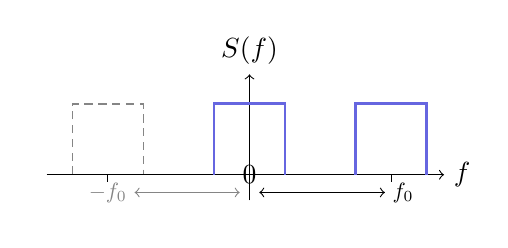
\begin{tikzpicture}[scale=0.9]

\node (null) at (0,0) {$0$};
\node (startY) at (0,-0.5) {};
\node (endY) at (0,1.75) {$S(f)$};
\node (startX) at (-3,0) {};
\node (endX) at (3,0) {$f$};


\draw[white!20!black!60, line width=0.5pt,densely dashed] (-2.5,0) -- (-2.5,1) -- (-1.5,1) -- (-1.5,0);

\draw [->] (startX) edge (endX);
\draw [->] (startY) edge (endY);
\draw[blue!80!black!60, line width=1pt] (-0.5,0) -- (-0.5,1) -- (0.5,1) -- (0.5,0);
\draw[blue!80!black!60, line width=1pt] (1.5,0) -- (1.5,1) -- (2.5,1) -- (2.5,0);


\node[scale=0.8,right=-1mm](offEnd)  at (2,-0.25) {$f_0$};
\node(offStart) at (0,-0.25) {};
\node[scale=0.8,white!20!black!60](offMirror) at (-2,-0.25) {$-f_0$};
\draw[<->,white!20!black!60]  (offStart) edge (offMirror);
\draw[<->]  (offStart) edge (offEnd);
\draw[line width=0.25pt] (2,0) -- (2,-0.1);
\draw[line width=0.25pt] (-2,0) -- (-2,-0.1);
\end{tikzpicture}\end{center}